\chapter{Anwendung des Frameworks auf jadice flow}
\label{chap:anwendung}

In diesem Kapitel wird ein Architektur-Refactoring am Produkt \emph{jadice flow} geplant und in theoretischer Ebene durchgeführt.
Dazu werden \acrfull{mmf} und \acrfull{arh} verwendet, welche den Prozess sowie auch dieses Kapitel in drei Phasen unterteilen.
Eine genauere Beschreibung des Frameworks ist in \cref{sec:mmf} zu finden.
Sehr abstrahiert und vereinfacht bestehen die Phasen aus den folgenden Aktivitäten:
\begin{itemize}
	\item In \cref{sec:durchführung-phase1} wird die Durchführung der ersten Phase in Form eines Architekturreviews mit den wichtigsten Stakeholdern beschreiben.
	\item Im Rahmen der zweiten Phase wird in \cref{sec:durchführung-phase2} nach adäquaten Migrationsstrategien gesucht.
	\item In \cref{sec:durchführung-phase3} wird in der dritten Phase nach profitablen Patterns und Best Practices gesucht.
\end{itemize}

\section{Phase 1 - Systemverständnis}
\label{sec:durchführung-phase1}

Das Ziel dieser Phase ist es, ein Verständnis des Systems aufzubauen.
Das ist zum einen auf Seite der Stakeholder wichtig.
Diese sollten spätestens nach dieser Phase wissen, welche \acrfullpl{qa} besonders wichtig für das System sind.
Zum anderen sollte der \gls{arh} nach dieser Phase durch Eingabe der \glspl{qa} ein Verständnis des Systems erlangen, das er in den nächsten Phasen zur Unterstützung der Entwickler bei Migration verwenden kann.
Um das Systemverständnis zu erlangen, wird in dieser Phase im Wesentlichen ein Architekturreview durchgeführt. 

\subsection{Qualitätsattribute}

Im ersten Schritt dieser ersten Phase werden die gewünschten \glspl{qa} des Systems gesammelt.
Hierfür wurde am 6. November 2023 in einer Fokusgruppe ein Architekturreview nach \Citet{SVAHNBERG20071893} wie in \cref{sec:methodik-architekturreview} beschrieben durchgeführt.
Teil dieser Gruppe waren vier Softwareentwickler beziehungsweise -Architekten, der \acrlong{po} und der Autor selbst in der Rolle des Moderators.
Leider war es nicht möglich, einen Kunden oder Nutzer des Produkts als Stakeholder für dieses Review zu organisieren.
Da das Entwicklungsteam jedoch regelmäßigen Kontakt mit Kunden hat, haben sie bestmöglich versucht, auch die Interessen der Kunden zu repräsentieren.
Aufgrund der ebenfalls in \cref{sec:methodik-architekturreview} beschriebenen Veränderungen an der Methodik von \Citet{SVAHNBERG20071893} wurde auch der geplante Zeitrahmen dieser Fokusgruppe auf zwei Stunden reduziert. Das liegt hauptsächlich daran, dass die letzten Phasen nicht erforderlich waren und alle Teilnehmer bereits vertraut mit dem Produkt und der Architektur und Funktionsweise des Systems waren.
Somit konnte nach einer kurzen Einführung in die verwendete Methodik ohne Verzögerung mit Schritt 2, dem Ordnen der \glspl{qa} nach Wichtigkeit, begonnen werden.

Im Rahmen dessen sollte jeder Teilnehmer seine Einschätzung darüber, welche die wichtigsten drei Sub-\glspl{qa} sind, per Nachricht mitteilen.
Die daraus resultierende Anzahl von Stimmen pro Sub-\gls{qa} ist in \cref{fig:qas-priority} dargestellt. 
% \begin{table}
  \centering
  \begin{tabular}{m{2.6cm} m{3.2cm} m{1.3cm} m{1.3cm}}
    \toprule
    \textbf{\gls{qa}} & \textbf{Sub-\gls{qa}} & \textbf{Anzahl Stimmen} & \textbf{Priorität} \\ \midrule
    Scalability & & 4 & 1\\ \hline

    \multirow{8}{=}[-0.1cm]{Maintainability} & Modularity & 4 & 2 \\
    & Monitorability & 2 & \\
    & Modifiabiltiy & 1 &  \\
    & Reusability & 1 &  \\
    & Testability & 1 &  \\
    & Analysability & 1 &  \\
    & Manageability & 1 &  \\
    & Understandability & 1 &  \\ \hline

    \multirow{2}{=}[-0.05cm]{Performance} & Time Behavior & 2 & 3 \\
    & Resource Utilization & 1 &  \\ \hline

   \multirow{5}{=}[-0.1cm]{Portability} & Deployability & 2 & 4 \\
   & Installability & 1 &  \\
   & Adaptability & 1 &  \\
   & Replaceability & 1 &  \\
   & Agility & 1 &  \\ \hline

    \multirow{3}{=}[-0cm]{Reliability} & Fault Tolerance & 1 & 5 \\
    & Recoverability & 1 & 6 \\
    & Availability & 1 &  \\ \hline

    Security & Confidentiality & 1 &  \\
    \bottomrule
  \end{tabular}
  \caption[Priorisierung der (Sub-) QAs durch Umfrage im Architekturreview]{
    Priorisierung der (Sub-) QAs durch Umfrage im Architekturreview in Phase 1 der Migration.
  }
  \label{tab:phase1-qas-priority}
\end{table}

\begin{figure}
	\centering
	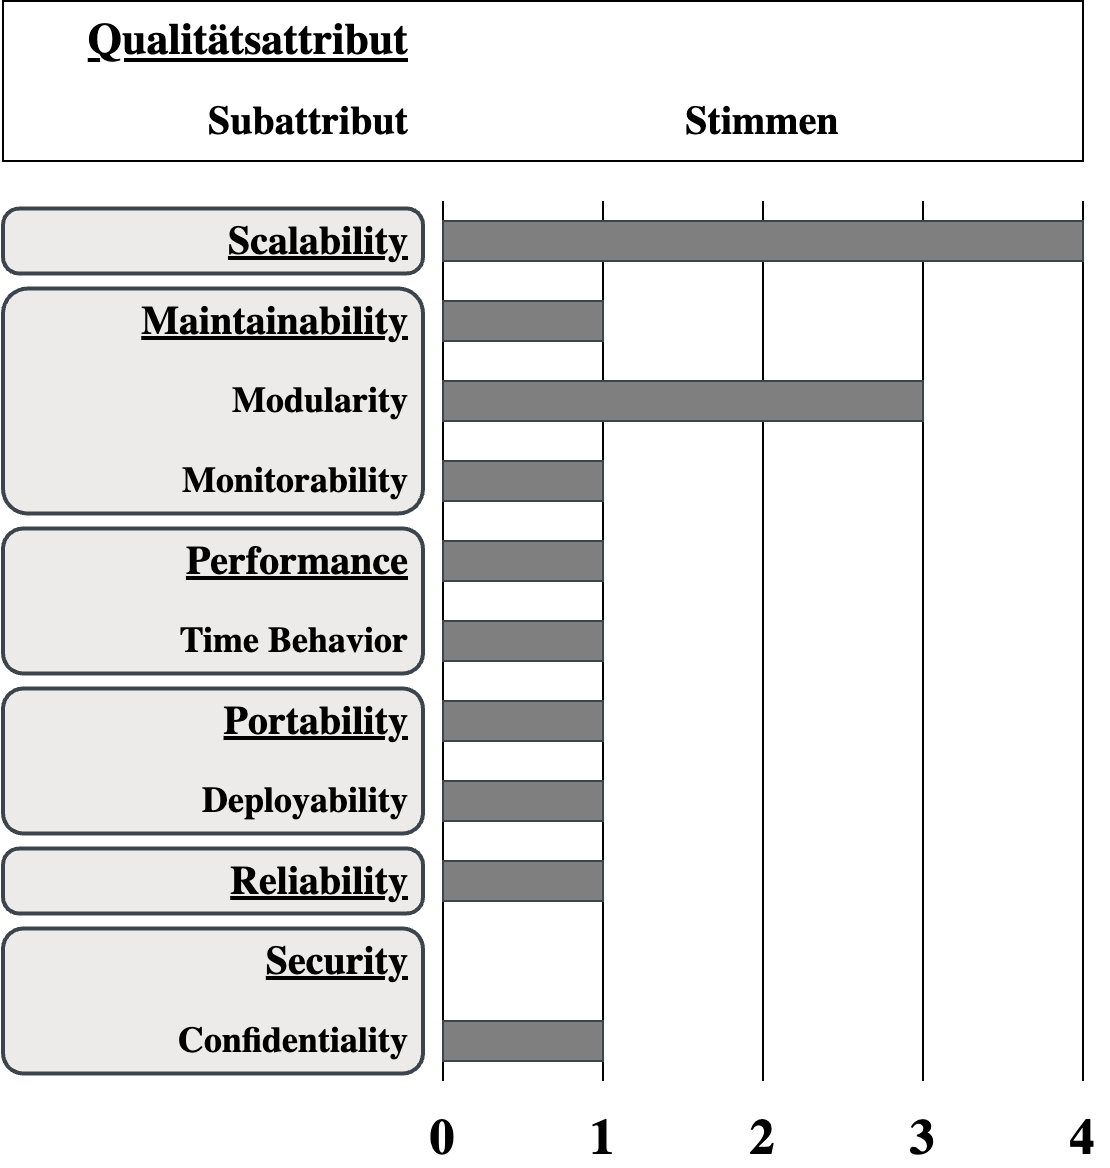
\includegraphics[width=0.8\textwidth]{qas-priority.drawio}
	\caption[Umfrageergebnisse wichtigste (Sub-) QAs im Architekturreview]{
		Umfrageergebnisse bei der Suche nach den wichtigsten (Sub-) QAs im Architekturreview in Phase 1 der Migration mit N = 5.
	}
	\label{fig:qas-priority}
\end{figure}
Dabei ist auffällig, dass auch  \acrlongpl{qa} Stimmen erhalten haben.
Das liegt daran, dass nicht alle Teilnehmer der Umfrage sich auf Sub-\glspl{qa} beschränkt haben, sondern auch die \glspl{qa} \emph{Performance}, \emph{Reliability}, \emph{Maintainability} und \emph{Portability} genannt wurden.
Auch wenn das nicht so vorgesehen war, wurde davon abgesehen, die Teilnehmer darauf hinzuweisen und es zu korrigieren, da die Ergebnisse nicht direkt zur Priorisierung der Attribute führen müssen.
Stattdessen wurden die Umfrageergebnisse und als vage Basis für eine freiere Diskussion über die Priorisierung verwendet. 
Deren Ergebnis war die schlussendliche Platzierung der sechs wichtigsten Sub-\glspl{qa}.
Im Folgenden werden diese erläutert.
\begin{enumerate}
	\item \textbf{\emph{Scalability}} ist ein \gls{qa} ohne Subattribute. Nach \Citet{master-daniel-koch} gibt es an, wie effizient ein System skaliert werden kann. Im Kontext von Microservices ist dabei vor allem die horizontale Skalierung relevant, welche die Skalierung über mehrere Instanzen von der Microservices beschreibt.
	\item \textbf{\emph{Modularity}} ist ein Subattribut von \emph{Maintainability}. Nach \Citet{master-daniel-koch} gibt es an, wie gut die Komplexität des Systems auf verschiedene Komponenten verteilt ist.
	\item \textbf{\emph{Time Behavior}} ist Subattribut von \emph{Performance}. Nach \Citet{master-daniel-koch} gibt es an, wie schnell ein System oder Teile eines Systems ankommende Anfragen beantworten.
	\item \textbf{\emph{Deployability}} ist ein Subattribut von \emph{Portability}. Nach \Citet{master-daniel-koch} gibt es an, wie einfach und schnell ein Produkt gebaut und ausgeliefert werden kann.
	\item \textbf{\emph{Fault Tolerance}} ist Subattribut von \emph{Reliability}. Nach \Citet{master-daniel-koch} gibt es an, inwieweit ein System wie erwartet funktionieren kann, obwohl in Teilen des Systems Fehler passieren.
	\item \textbf{\emph{Recoverability}} ist ebefalls Subattribut von \emph{Reliability}. Nach \Citet{master-daniel-koch} gibt es an, inwieweit ein System nach einem Ausfall wieder den Zustand vor dem Ausfall herstellen kann, sowie Daten erhalten kann.
\end{enumerate}
Die genaue Anzahl der wichtigsten (Sub-)Attribute war nicht vor dem Termin definiert, sondern wurde ebenfalls von der Gruppe diskutiert (in einem späteren Schritt) und gemeinsam auf sechs festgelegt.
Der gesamte Prozess der Umfrage und anschließender Diskussion, um die Prioritäten der Attribute zu setzen, dauerte etwa 15 Minuten und entsprach somit der geplanten Zeit.

Im nächsten Schritt war die Aufgabe, für jedes dieser (Sub-) \glspl{qa} zwei Szenarien zu definieren, die das Attribut gut und auf verschiedene Arten beschreiben.
Es wurde keine spezielle Methodik angewandt, sondern in einer offenen Diskussion der gesamten Gruppe von verschiedenen Teilnehmern nacheinander für die Attribute Szenarien vorgeschlagen und anschließend überarbeitet oder teilweise auch abgelehnt.
Nach einer Diskussionszeit von etwa 35 Minuten ergaben sich die Szenarien, die in  \cref{fig:scenarios} abgebildet sind. 

\begin{figure}
	\centering
	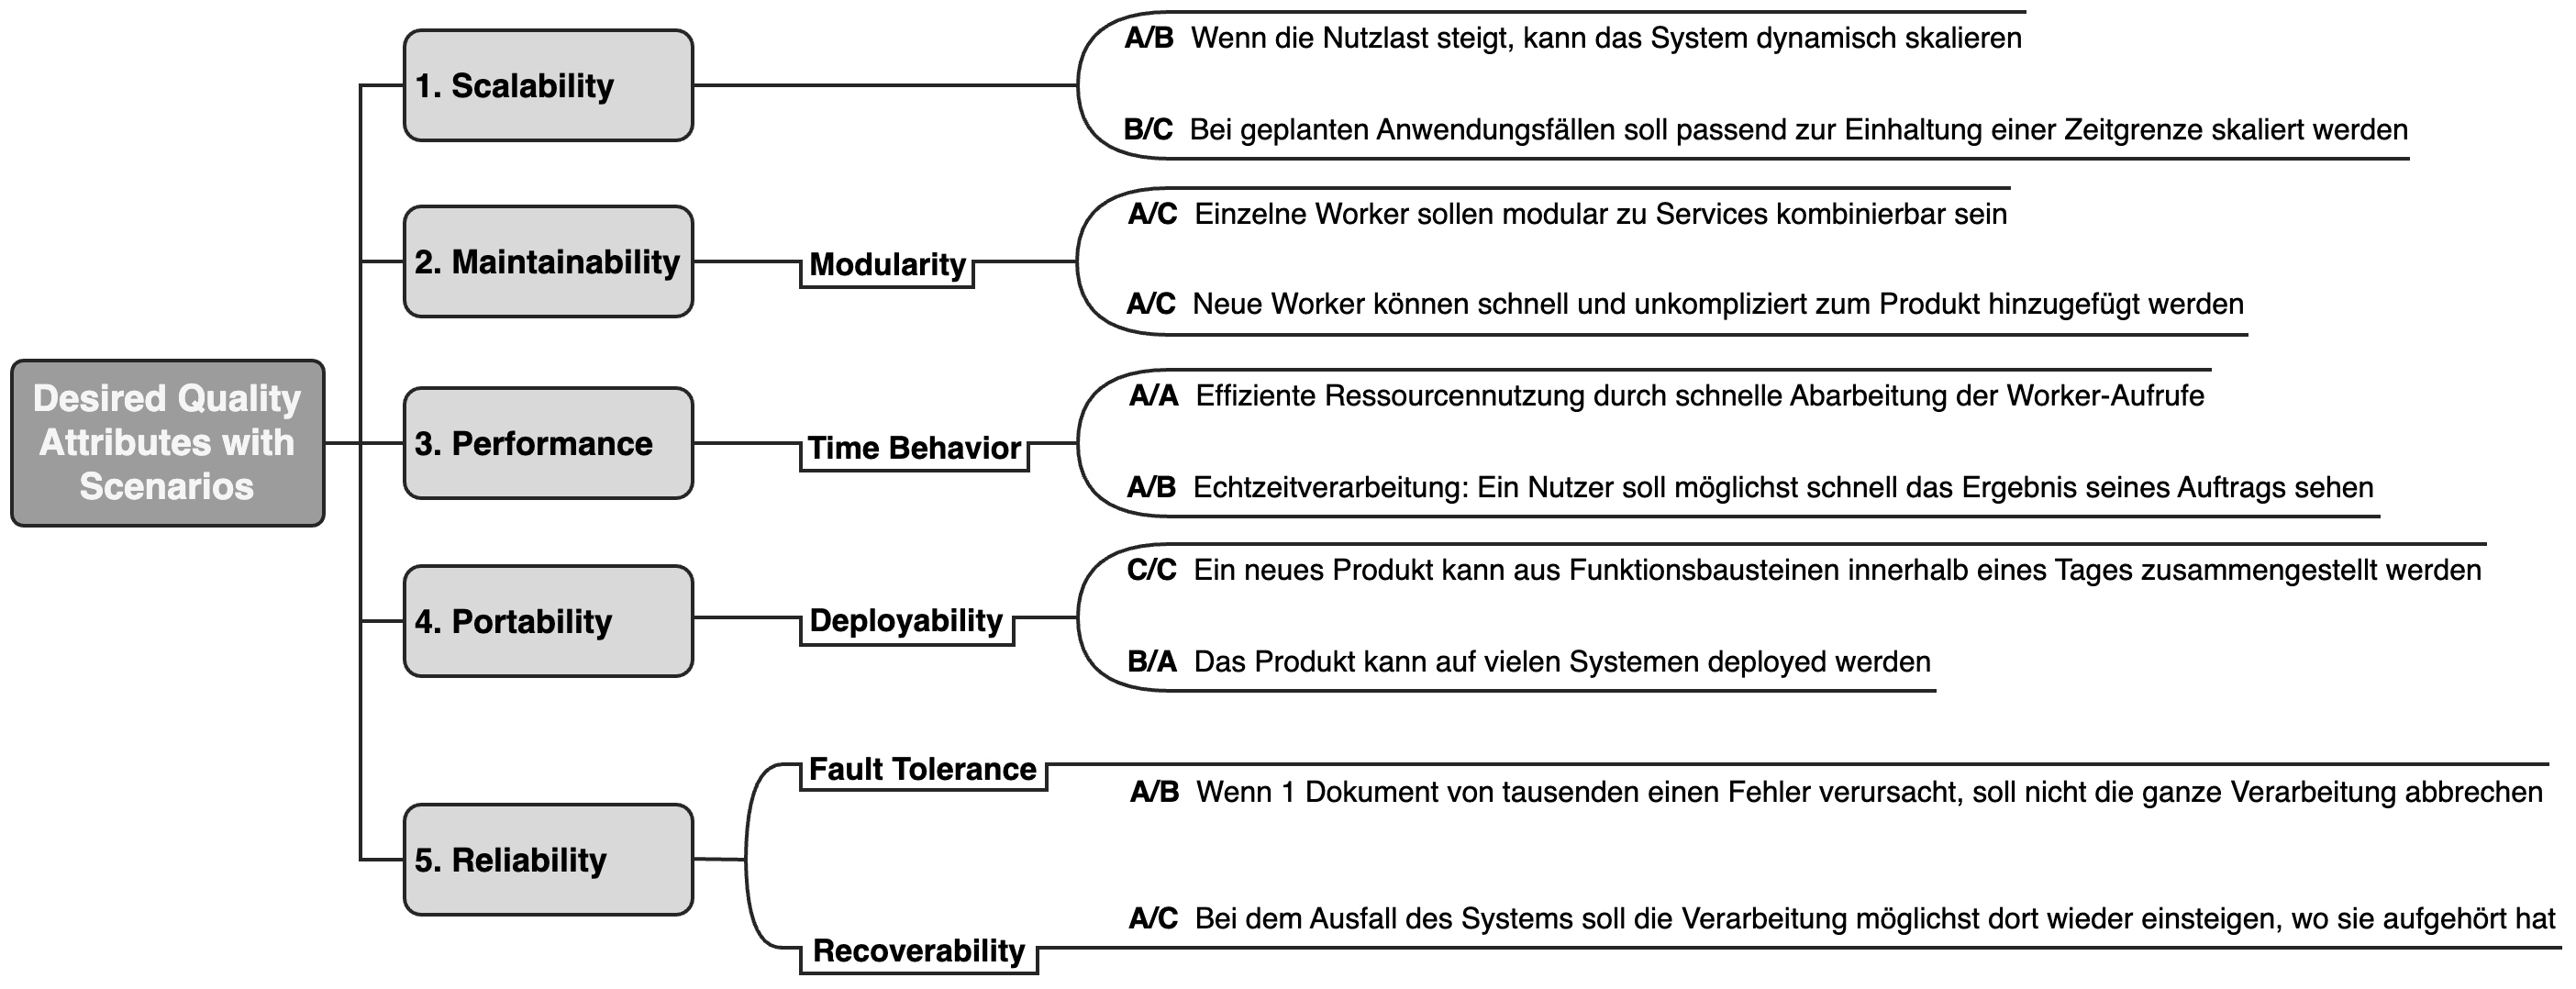
\includegraphics[angle=270,width=\textwidth]{scenarios.drawio}
	\caption[Utility Tree mit im Architekturreview ermittelten Qualitätsanforderungen und Szenarien]{
		Der Utility Tree mit Szenarien, die aus dem in Phase 1 durchgeführten Architekturreview resultieren.
		Von oben nach unten enthält der Baum folgende Elementarten: [1] Wurzel (ohne Bedeutung), [2] \gls{qa}, [3] Subattribut, [4] Beurteilung des Szenarios hinsichtlich Wichtigkeit und technischer Schwierigkeit, [5] Szenariobeschreibung.
	}
	\label{fig:scenarios}
\end{figure}

Wie aus der Abbildung ersichtlich, wurden für jedes (Sub-)Attribut mit Ausnahme von \emph{Fault Tolerance} und \emph{Recoverability} jeweils zwei Szenarien erstellt.
Dies hat zwei Gründe.
Zum einen wurden für diese Subattribute keine ausreichend unterschiedlichen Szenarien gefunden. 
Zum anderen wurde in diesem Fall ein Szenario als ausreichend betrachtet, da Reliability das einzige QA ist, für das mehrere Subattribute eingeschlossen wurden. 
Darüber hinaus ist es das am geringsten priorisierte Attribut.

Um zusätzliche eine Priorisierung der Szenarien vornehmen zu können, sieht der \gls{arh} jeweils eine dreistufige Bewertung der Szenarien hinsichtlich ihrer Wichtigkeit und ihrer technischen Schwierigkeit vor.
Diese wurde im nächsten Schritt vorgenommen.
Dabei haben die Teilnehmer die Szenarien der Reihe nach betrachtet und ihre Wichtigkeit und technische Schwierigkeit diskutiert.
Nicht immer waren alle anfangs einer Meinung, doch schlussendlich konnte nach etwa 35 Minuten für jedes Szenario Konsens gefunden werden und diese Phase abgeschlossen werden.

Da die Vollendung einiger Schritte länger gedauert hat als geplant, waren am Ende dieses Termins nur noch wenige Minuten übrig.  
Vor allem der dritte Schritt nach \Citet{SVAHNBERG20071893} war dafür ausschlaggebend, da für alle Sub-Schritte zusammen nur 60 Minuten eingeplant waren, jedoch das Sammeln der Szenarien und das Bewerten dieser (also zwei von drei Sub-Schritten) schon 70 Minuten in Anspruch nahmen.
Daher wurde entschieden, die restlichen Punkte in einer weiteren Sitzung in der nächsten Woche zu bearbeiten.

Am 14. November 2023 wurde dann der zweite Teil des Architekturreviews durchgeführt.
Anwesend waren dieselben Personen.
Da bei diesem Treffen ein neuer Blickwinkel auf die Thematik möglich gewesen wäre, wurden zunächst zehn Minuten darauf verwendet, die bereits vorhandenen Szenarien und die Bewertung dieser hinsichtlich Wichtigkeit oder technischer Schwierigkeit erneut zu überprüfen und Raum für mögliche Änderungen zu schaffen.
Es wurden jedoch keine Änderungen vorgenommen und die Teilnehmer bestätigten lediglich erneut die bereits vorhandenen Szenarien.

Anschließend wurde wie geplant damit fortgefahren, die Szenarien weiteren \glspl{qa} zuzuordnen.
Oft werden können nämlich trotz der Erstellung eines Szenarios für ein bestimmtes \gls{qa} weitere \glspl{qa} damit assoziiert werden.
Deswegen wurde erneut jedes Szenario der Reihe nach betrachtet und diskutiert, welche weiteren (Sub-) Attribute darauf zutreffen könnten.
Nach etwa 15 Minuten Diskussion waren alle Szenarien behandelt und für jedes einstimmig geklärt, welche weiteren Subattribute damit assoziiert werden.
Diese werden folgend im Bezug auf die jeweiligen Szenarios sekundäre \glspl{qa} genannt, wohingegen ein \gls{qa}, für das das Szenario erstellt wurde, primäres \gls{qa} genannt wird.
Die resultierenden Assoziationen sind in der \cref{tab:scenarios} aufgeführt.

\begin{table}[!h]
  \centering
  \begin{tabular}{ m{2,3cm} m{6cm} m{0.7cm} m{2,5cm} p{0.7cm} }
    \toprule
    \textbf{Name} & \textbf{Beschreibung} & \textbf{W/S} & \textbf{\glspl{qa}} & \textbf{MS} \\
    \midrule
    Dynamische Ska\-lier\-bar\-keit & Wenn die Nutzlast steigt, kann das Sys\-tem dynamisch skalieren & A/B & Scalability, Re\-source Uti\-li\-za\-tion, Adaptability, Execution Cost & \advantage \\ \hline
    Statische Ska\-lier\-bar\-keit & Bei geplanten Anwendungsfällen soll passend zur Einhaltung einer Zeitgrenze skaliert werden & B/C & Scalability, Resource Utilization, Time Behavior & \advantage \\  \hline
    Jobtemplates& Einzelne Worker sollen modular zu Services kombinierbar sein & A/C & Modularity, Reusability & - \\ \hline
    Neue Worker& Neue Worker können schnell und un\-kom\-pliziert zum Produkt hinzugefügt werden & A/C & Modularity, Reusability & \advantage  \\ \hline
    Schnelle Ab\-ar\-bei\-tung & Effiziente Ressourcennutzung durch schnelle Abarbeitung der Worker-Auf\-rufe  & A/A & Time Behavior, Resource Uti\-li\-za\-tion & \disadvantage \\ \hline
    \glqq Echtzeit\grqq{}-Verarbeitung & Ein Nutzer soll möglichst schnell das Ergebnis seines Auftrags sehen & A/B & Time Behavior & \disadvantage \\ \hline
    Einfaches De\-ploy\-ment & Ein neues Produkt kann aus Funk\-tions\-bausteinen innerhalb eines Tages zusammengestellt werden &C/C & Deployability, Modularity, Agility & \disadvantage \\ \hline
    Platform-unabhängigkeit& Das Produkt kann auf vielen Systemen deployed werden & B/A & Deployability, Installability & \advantage \\ \hline
    Fehlerto\-leranz Massen\-ver\-ar\-beitung & Wenn 1 Dokument von tausenden einen Fehler verursacht, soll nicht die ganze Verarbeitung abbrechen & A/B & Fault-Tolerance &\advantage \\ \hline
    Erholen nach Sys\-tem\-ausfall & Bei dem Ausfall des Systems soll die Verarbeitung möglichst dort wieder einsteigen, wo sie aufgehört hat & A/C & Recoverability & - \\
    \bottomrule
  \end{tabular}
  \caption[Im Architekturreview ermittelte Qualitätsanforderungen und Szenarien]{
    Szenarien, die aus dem in Phase 1 durchgeführten Architekturreview resultieren.
    \emph{W/S} gibt die Wichtigkeit/Schwierigkeit der Szenarien in drei Stufen an (A steht für sehr wichtig und sehr schwierig).
    \emph{\glspl{qa}} gibt die Assoziation der Szenarien zu bestimmten \acrfullpl{qa} an; zuerst genannte sind primäre \glspl{qa}, folgende sekundäre \glspl{qa}.
    \emph{MS} gibt die Einschätzung darüber an, ob das jeweilige Szenario von einer Microservices-Architektur profitiert.
  }
  \label{tab:scenarios}
\end{table}


Damit wurde der für die Extraktion der Qualitätsanforderungen des Systems relevante Teil des Architekturreviews abgeschlossen.
Zusammenfassend kann gesagt werden, dass die Phase größtenteils wie geplant durchgeführt werden konnte.
An einigen Stellen sind die verschiedene Schritte etwas verschmolzen oder es wurde kurz zu vorherigen Schritten zurückgesprungen, was jedoch vollkommen normal ist und auch beispielsweise in \gls{atam} von \Citet{kazman_2000} als gängige Praxis beschrieben wird.
So wurde in diesem Fall beim Erstellen der Szenarien entschieden, bis zu welcher Priorität die \glspl{qa} mit Szenarien versehen werden, obwohl die Wahl der Anzahl der wichtigsten tatsächlich für den vorherigen Schritt geplant war.
Die Beteiligung der Teilnehmer war komplett ausgeglichen, aber jeder hat regelmäßig etwas beigetragen.
Es kann angenommen werden, dass das Ergebnis von allen Teilnehmern ausreichend geformt wurde und dass keine einseitige Beeinflussung vorliegt.

\subsection{Architekturbewertung}

Neben de Erfassung der wichtigsten Szenarien und \glspl{qa} hatte die Fokusgruppe als sekundäres Ziel, die Wahl der Architektur für \emph{jadice flow} zu bewerten. 
Diese Bewertung wurde ebenfalls in der zweiten Sitzung des Architekturreviews durchgeführt und entspricht dem vierten Schritt \emph{Assessment} der ersten Phase des \gls{arh}.
Da dieser Schritt jedoch noch nicht im Werkzeug implementiert ist, wurde er manuell durchgeführt.
Im Gegensatz zu vorherigen Schritten der ersten Phase ist dieser nicht relevant für die nächsten Phasen, weshalb es kein Problem ist, den \gls{arh} hierbei nicht zu verwenden.
In diesem Schritt wurde die Frage diskutiert, ob eine \acrlong{msa} individuell für jedes Szenario vorteilhaft ist im Vergleich zu einer monolithischen Architektur.
Hierbei wurde in drei Stufen unterschieden:
\begin{itemize}
	\item \advantage\hspace*{0.1cm}: Dieses Szenario profitiert wesentlich mehr von einer \gls{msa} als von einer monolithischen Architektur.
	\item \disadvantage\hspace*{0.1cm}: Dieses Szenario profitiert wesentlich mehr von einer monolithischen Architektur als von einer \gls{msa}.
	\item \hspace*{0.27cm}-\hspace*{0.27cm}: Dieses Szenario profitiert in verschiedenen Punkten sowohl von einer \gls{msa} als auch von einer monolithischen Architektur, wobei sich beide Seiten ungefähr gleichen.
\end{itemize}
Bei Szenarios wie beispielsweise den des \emph{Scalability} Attributs war es nicht schwer, Konsens zu finden, da die Möglichkeit der Skalierung auf Service-Ebene einer der größten Vorteile von \glspl{msa} gegenüber Monolithen ist.
In anderen Fällen jedoch war es schwieriger, abzuwägen, ob die Vorteile einer \gls{msa} oder die eines Monolithen überwiegen.
Schlussendlich konnte jedoch in Form von offener  Diskussion für jedes Szenario einstimmig geklärt werden, welche der drei Optionen gewählt werden sollte, sodass keine Abstimmungen notwendig waren.

Das Ergebnis dieser Einschätzungen ist ebenfalls in \cref{tab:scenarios} zu sehen.
Insgesamt wurde eine \gls{msa} in fünf Fällen als vorteilhaft und nur in drei Fällen als unvorteilhaft bewertet. 
Des Weiteren ist zu beachten, dass die Szenarien in der Tabelle nach der Wichtigkeit der primären \glspl{qa} sortiert sind und die obersten beiden Szenarien die Hauptfaktoren für die Migration zu einer Microservices-Architektur waren.
Durch die Überlegenheit der \gls{msa}-Favorisierungen und dass diese verstärkt bei den wichtigsten \glspl{qa} vorliegen kann diese Metrik die Entscheidung zur Migration zu einer \gls{msa} bestätigen.

\section{Phase 2 - Strategieplanung}
\label{sec:durchführung-phase2}

In dieser Phase werden die Ergebnisse der Phase 1 in Form von \glspl{qa} beziehungsweise Szenarien genutzt, um eine passende Migrationsstrategie zu finden.
Dazu wurden die in \cref{tab:scenarios} dargestellten Szenarien bereits in den \gls{arh} eingegeben.
Zusätzlich werden in dieser Phase Filterkriterien definiert.
Mit deren Hilfe wird dann schlussendlich eine Liste von Migrationsstrategien vorgeschlagen, welche folgend analysiert wird.

\subsection{Filterselektion}
Damit bei der Suche nach Migrationsmethoden möglichst gut zum Zielsystem und den Vorstellungen der Architekten passende Ergebnisse vorgeschlagen werden, bietet der \gls{arh} neben der Konfiguration der Szenarien noch eine weitere Art, die Ergebnisse zu filtern und ordnen: Die Filter, die in diesem Abschnitt konfiguriert werden.
Dabei kann für jede der Eigenschaften aus \cref{tab:phase2-filter} eine dieser drei Präferenzen angegeben werden:
\begin{itemize}
	\item \textbf{Include:} Methoden, die die jeweilige Eigenschaft haben, werden höher platziert.
	\item \textbf{Neutral:} Ob Methoden die jeweilige Eigenschaft haben, wirkt sich nicht auf ihre Platzierung aus.
	\item \textbf{Exclude:} Methoden, die die jeweilige Eigenschaft nicht haben, werden höher platziert.
\end{itemize}


Für die Wahl der Filter für das Refactoring von \emph{jadice flow} haben \gls{po} und der Autor alle Filter betrachtet und die wichtigsten relevanten ausgewählt.
Diese sind \cref{tab:phase2-filter} farblich markiert.
Bewusst stammen die meisten gewählten Filter aus der Kategorie \emph{System Properties} gewählt. da diese als am ausschlaggebendsten für das System 
Der Grund dafür ist, dass bereits ohne Filtereinstellung das wichtigste 

Um bestmögliche Ergebnisse zu erhalten und dabei eine breite Abdeckung zu erhalten, wird das Suchverfahren mehrfach mit verschiedenen Filtereinstellungen wiederholt.

\begin{table}
  \centering
  \begin{tabular}{m{2cm} m{2cm} m{9cm}}
    \toprule
    \textbf{Kategorie} & \textbf{Subkategorie} & \textbf{Eigenschaften} \\
    \midrule
    Quality Preferences & System Properties & Autonomy, Cohesion, Complexity, Coupling, Granularity, Isolation, Technology Heterogenity \\ \hline
    \multirow{4}{=}[-1cm]{Input Preferences} & Domain Artifacts &  Documentation, Human expertise, Ontology, Version Control System \\ \cline{2-3}
    & Runtime artifacts & Log traces, User-Application interactions \\ \cline{2-3}
    & Model artifacts & Activity diagram, Business process model, Class diagram, Custom model, Data flow diagram, Entity model, State machine diagram, Use case model \\ \cline{2-3}
    & Executables & API / Interface, Database file, Source code (Java), Source code (No specification), Source code (Python), Test cases \\ \hline
    \multirow{6}{=}[-1.9cm]{Process Preferences} & Directions & Bottom-up, Mixed, Top-down \\ \cline{2-3}
    & Levels of automation & Automatic, Manual, Semi-automatic \\ \cline{2-3}
    & Analysis types & Dynamic, Historic, Lexical, Static \\ \cline{2-3}
    & Techniques & Clustering, Custom heuristics, Data-flow driven, Domain-Driven Design, Execution-trace modeling, General guidelines, Genetic algorithm, Graph-based, Machine Learning, Multi-Tenancy, Performance modeling, Scenario analysis, Wrapping / Black Box \\ \cline{2-3}
    & Process Strategy & Continuous Evolution, Extension, Greenfield, Refactor, Rewrite / Rebuild, Strangler \\ \cline{2-3}
    & Atomar Unit & Business Capability, Class, Entity, Function, Functionality, Interface, Other \\ \hline
    Output Preferences & Representation & Guideline / Workflow, List of services, Source code, Splitting recommendations, Visualization \\ \hline
    \multirow{4}{=}[-1cm]{Usability Preferences} &Validation methods & Case study, Experiment, Industry, No validation \\ \cline{2-3}
    & Accuracy of \gls{sia} & High, Medium, Low, Not available \\ \cline{2-3}
    & Tool supports &  No tool support \\ \cline{2-3}
    & Tool types & Database, Decomposition, Dynamic Analysis, Java, Open Source, Other, Reverse Engineering, Static Analysis, Visualization \\
    \bottomrule
  \end{tabular}
  \caption[Mögliche Filter des \gls{arh} in Phase 2]{
    Mögliche Filter des \gls{arh} in Phase 2.
  }
  \label{tab:phase2-filter}
\end{table}





Die Qualität dieser Filterfunktion soll ebenfalls in dieser Arbeit evaluiert werden, weshalb folgend in \cref{sec:phase2-ergebnisdurchsicht} die Ergebnisse verschiedener Filter betrachtet und verglichen werden.
Dafür wurden die Filter für das Refactoring von \emph{jadice flow} wie folgt gewählt.
Das Vorgehen ist in \cref{feldnotiz:1} dokumentiert.

\subsection{Suchergebnisbetrachtung}
\label{sec:phase2-ergebnisdurchsicht}

Die Filter, die im vorherigen Abschnitt gewählt wurden, werden in diesem Abschnitt angewendet, um jeweils geordnete Listen von Ergebnissen zu erhalten.
In Tabelle TODO werden

\begin{table}[!ht]
	\centering
	\begin{tabular}{l c c c}
		\toprule
    \textbf{Publikation} & \multicolumn{3}{c}{\textbf{Matches}} \\
     & \textbf{Insgesamt} & \textbf{\gls{qa}} & \textbf{\gls{sp}} \\ \midrule
    \multicolumn{4}{c}{\textbf{Alle Filter (15)}} \\ \midrule
    \Citet{arh-result-no-filter-1} & 15/32 & 11/17 & 0/5 \\ \hline
    \Citet{arh-result-no-filter-3} & 13/32 & 7/17  & 1/5  \\ \hline
    \Citet{arh-result-no-filter-2} & 12/32 & 7/17  & 2/5  \\ \hline
    \Citet{arh-result-no-filter-4} & 11/32 & 7/17  & 0/5  \\ \hline
    \Citet{arh-result-no-filter-5} & 11/32 & 7/17  & 0/5  \\ \midrule
		\multicolumn{4}{c}{\textbf{Wichtigste Filter (9)}} \\ \midrule
		\Citet{arh-result-no-filter-1}        & 14/26 & 11/17 & 0/3 \\ \hline
		\Citet{arh-result-no-filter-3}        & 13/26 & 7/17  & 1/3  \\ \hline
		\Citet{arh-result-no-filter-2}        & 11/26 & 7/17  & 1/3  \\ \hline
		\Citet{arh-result-important-filter-4} & 10/26 & 6/17  & 1/3  \\ \hline
    \Citet{arh-result-no-filter-4}        & 10/26 & 7/17  & 0/3  \\ \hline
    \textbf{\Citet{arh-result-no-filter-5}}        & 10/26 & 7/17  & 0/3  \\ \hline
    \textbf{\Citet{arh-result-important-filter-7}}        & 10/26 & 5/17  & 1/3  \\ \midrule
    \multicolumn{4}{c}{\textbf{Keine Filter (Nur \glspl{qa})}} \\ \midrule
    \Citet{arh-result-no-filter-1} & 11/17 & 11/17 & - \\ \hline
    \Citet{arh-result-no-filter-2} & 7/17  & 7/17  & - \\ \hline
    \Citet{arh-result-no-filter-3} & 7/17  & 7/17  & - \\ \hline
    \Citet{arh-result-no-filter-4} & 7/17  & 7/17  & - \\ \hline
    \Citet{arh-result-no-filter-5} & 7/17  & 7/17  & - \\ \bottomrule
	\end{tabular}
	\caption[Surchergebnisse des ARH von Migrationsverfahren mit verschiedenen Filtern]{
		Ergebnisse der Suche mit ARH nach Migrationsverfahren mit verschiedenen Filtern, wie in \cref{sec:filterselektion} näher beschrieben, nach Matches sortiert.
		Insgesamte Matches, \gls{sp} Matches und \gls{qa} Matches entsprechen den im \gls{arh} angezeigten Matches.
	}
	\label{tab:phase2-filter-results}
\end{table}


Suche nur mit QA
Suche mit allen Filtern
Suche nur mit wichtigsten Filtern
Manuelle Suche ohne Priorisierung des Systems

\section{Phase 3a - Architekturplanung}
\label{sec:durchführung-phase3}